% IEEE QCE submission skeleton — Entangled Equilibria
% Build: latexmk -pdf main.tex   (or upload paper/ to Overleaf; IEEEtran is built in)
% Convention: \todo{...} marks prose to be written; all numbers already present
% are REAL (from results/ artifacts, cited in comments beside each).
\documentclass[conference]{IEEEtran}
\usepackage{amsmath,amssymb}
\usepackage{graphicx}
\usepackage{booktabs}
\usepackage{xcolor}
\usepackage[colorlinks=true,linkcolor=blue,citecolor=blue,urlcolor=blue]{hyperref}
\graphicspath{{figs/}}
\newcommand{\todo}[1]{\textcolor{red}{[TODO: #1]}}
\newcommand{\ket}[1]{\ensuremath{|#1\rangle}}

\title{Entanglement Topology and Noise Determine Quantum Advantage in
$N$-Player Trading Games:\\ Simulation Landscape and Hardware Validation}

\author{%
\IEEEauthorblockN{Prithvi Raghu}
\IEEEauthorblockA{VIT Vellore\\prithviraghu080706@gmail.com}
\and
\IEEEauthorblockN{Aasa Singh Bhui}
\IEEEauthorblockA{VIT Vellore\\\todo{email}}
}

\begin{document}
\maketitle

\begin{abstract}
% Real numbers: results/hardware-scaling/2026-07-16T074134Z/, README §9.
We extend the two-player quantum Hawk--Dove trading game of Khan et al.\ to
$N$ players under five entanglement topologies (GHZ, W, ring, star,
fully connected) using the Eisert--Wilkens--Lewenstein (EWL) protocol, and map
how topology, player count, and depolarizing noise jointly determine quantum
advantage. Three findings organize the landscape. First, at the maximally
entangled point the cooperative quantum profile pays exactly $V/N$ against a
classical Nash payoff of $1/N$ --- a constant $4\times$ multiplier for $V=4$
--- but it is a self-enforcing equilibrium only at $N=3$. Second, under noise
the two natural robustness criteria \emph{disagree}: GHZ --- the only
topology whose cooperative profile is a pure equilibrium ($N{=}2,3$) ---
loses it at finite noise yet retains the largest mean advantage at small $N$
(an ordering that matched-gate-count controls attribute to circuit gate
budgets rather than entanglement structure, W's $\sim$2.5$\times$ per-gate
robustness excepted), while
W never crosses zero in the mean but hides position-locked per-player losses
that strategy adaptation does not repair. Third, on an IBM Heron r2 processor
(ibm\_fez), a scaling
experiment at $N=3,4,5$ on one pinned qubit chain retains
99.4\%/98.7\%/98.1\% of the ideal advantage $3/N$ after readout mitigation and
zero-noise extrapolation. A single depolarizing parameter fitted to the
$N{=}3$ point alone --- the registered primary prediction --- matches
$N{=}4$ to 0.004 but over-predicts $N{=}5$ by 0.010, a registered
$\approx$5$\sigma$ deviation that reproduces across runs; a
per-two-qubit-gate decay law leads the registered model comparison, with the
depolarizing fit as its physical interpretation. The mean-payoff observable is first-order
insensitive to single bit-flips, so the advantage decays several times slower
than state fidelity --- a structural robustness with direct consequences for
quantum market design.
\end{abstract}

\begin{IEEEkeywords}
quantum games, Nash equilibrium, EWL protocol, entanglement topology, NISQ,
error mitigation, quantum finance
\end{IEEEkeywords}

% =============================================================================
\section{Introduction}\label{sec:intro}

Financial markets are coordination problems with adversarial payoffs. When
traders compete over a scarce asset, each chooses between an aggressive
position --- capturing the full value if unopposed --- and a cooperative one
that shares value reliably. The Hawk--Dove game formalizes this tension: the
aggressive pure equilibria are asymmetric and unstable, the symmetric mixed
equilibrium pays strictly less than mutual cooperation, and the all-Hawk
outcome destroys value for every participant at once. Market crashes are the
macroscopic version of that last cell --- a tragedy of the commons in which
individually rational aggression, played by everyone, leaves each player worse
off than cooperation would have. Classical remedies are external to the game:
trust between counterparties, a trusted intermediary, or regulation that taxes
defection.

Quantum game theory offers a different lever. In the
Eisert--Wilkens--Lewenstein (EWL) protocol~\cite{eisert1999}, strategies live
in SU(2) and players' qubits are entangled before any move is made; the
correlation structure of the shared state then changes what is
self-enforcing. The celebrated two-player result is a quantum Nash equilibrium
that is simultaneously symmetric and Pareto-optimal: cooperation pays the same
as mutual trust but is enforced by interference rather than by an
institution. For market mechanisms --- carbon-trading schemes, order-book
architectures, DeFi protocols --- this suggests replacing a regulatory cost
with a physical correlation.

Khan et al.~\cite{khan2025} demonstrated a quantum Nash-equilibrium advantage
for the two-player trading game on ion-trap hardware. Two players, however,
admit exactly one entanglement geometry. Real markets are networks: the
\emph{topology} of who is correlated with whom is a design variable, and each
topology induces a different interference structure, different equilibria, and
a different response to decoherence. Varsamis et al.~\cite{varsamis2025}
studied $N$-player entanglement operators and scalability on IBM hardware;
our contribution is orthogonal: we fix a financially interpreted game and
chart how \emph{topology $\times$ player count $\times$ noise} determine both
the magnitude and the equilibrium status of the quantum advantage, then test
the resulting noise model against registered predictions on hardware.

Our contributions:
\begin{enumerate}
  \item \textbf{Advantage landscape.} The complete $(N,\text{topology})$
  advantage map for $N=2$--$6$ over five topologies, including the finding
  that the fixed GHZ-derived cooperative profile $(Q_N,\dots,Q_N)$ is a pure
  Nash equilibrium only at $N=3$; for $N\ge4$ a unilateral Hawk deviation
  profits even without noise. % compute_advantage: dev 2.0 vs 1.0 (N=4), 2.618 vs 0.8 (N=5)
  \item \textbf{Noise-robustness dichotomy.} Under depolarizing noise the
  equilibrium criterion and the advantage-magnitude criterion order topologies
  \emph{differently}; noise also breaks player symmetry, producing
  position-locked per-player disadvantage that follows the entangler's gate
  ordering (proved by a wiring-permutation experiment) and that independent
  best-response adaptation fails to repair. Matched-gate-count and
  compilation controls attribute the advantage-magnitude ordering within the
  XX-product family (GHZ/ring/star/fully connected) to circuit gate budgets
  rather than entanglement structure; W's $\sim$2.5$\times$ per-gate
  robustness is the surviving structural effect.
  % docs/findings/2026-07-16-topology-vs-implementation-controls.md
  \item \textbf{Predictive hardware validation.} An $N=3,4,5$ scaling
  experiment on ibm\_fez (one pinned chain, one batch job) with tensored
  readout mitigation and cz-fold zero-noise extrapolation retains
  98--99\% of the ideal advantage $3/N$; a one-parameter depolarizing model
  fitted at $N{=}3$ --- the registered primary prediction --- matches
  $N{=}4$ to 0.004 while its $N{=}5$ miss (0.010, $\approx$5$\sigma$,
  reproduced) leaves a registered per-two-qubit-gate decay baseline leading
  the model comparison. We identify the
  mechanism --- first-order insensitivity of the mean payoff to single
  bit-flips --- that makes the advantage more noise-robust than the state.
  \item \textbf{Reproducible pipeline.} An open-source harness with
  circuit-identity gates, a mandatory device-model dress rehearsal before any
  hardware submission, and crash-safe job recovery.
\end{enumerate}

% =============================================================================
\section{Background and Related Work}\label{sec:background}

\subsection{The Hawk--Dove trading game}
% payoff matrix + financial mapping: README §3.1
Two traders compete over a single asset of value $V$; conflict costs $C$.
Hawk is the aggressive position (a short: it captures the full value if
unopposed but destroys value in symmetric conflict); Dove is the cooperative
position (a long: it shares value reliably). The payoff matrix is
\begin{center}
\renewcommand{\arraystretch}{1.15}
\begin{tabular}{l|cc}
 & \textbf{opp.\ Dove (long)} & \textbf{opp.\ Hawk (short)}\\
\hline
\textbf{you Dove (long)} & $V/2,\ V/2$ & $0,\ V$\\
\textbf{you Hawk (short)} & $V,\ 0$ & $(V{-}C)/2,\ (V{-}C)/2$\\
\end{tabular}
\end{center}
We fix $V{=}4,\ C{=}3$ throughout (the repo's live convention,
\texttt{src/config.py}). The two pure Nash equilibria --- one Hawk, one Dove
--- are asymmetric and unstable, requiring coordination on who takes which
role. The symmetric classical outcome is a mixed equilibrium in which each
player plays Hawk with probability $V/C$; its expected payoff is strictly
below the mutual-Dove payoff $V/2$. When everyone plays Hawk, both pay
$(V{-}C)/2$: value destruction every participant at once.

\subsection{The EWL protocol and its $N$-player extension}
The EWL quantization~\cite{eisert1999} embeds strategies in SU(2) and
entangles qubits before strategy application:
\begin{equation}
\ket{\psi_{\text{out}}} = J^\dagger \left(\bigotimes_{j=1}^{N} U_j\right) J\, \ket{0}^{\otimes N},
\qquad
J = e^{i \frac{\gamma}{2} X^{\otimes N}},
\end{equation}
with maximal entanglement at $\gamma=\pi/2$~\cite{benjamin2001,flitney2002}.
The $N$-appropriate quantum strategy generalizes to
$Q_N = U(0, \pi/N, \pi/N)$; at $\gamma=\pi/2$ the profile $(Q_N,\dots,Q_N)$
maps $\ket{0}^{\otimes N}$ back to $\ket{0}^{\otimes N}$ exactly, so the ideal
output is a single computational basis state at every $N$.

\subsection{Relation to prior $N$-player hardware work}
Varsamis et al.~\cite{varsamis2025} study $N$-player entanglement operators
and their scalability on IBM hardware generically --- characterising the
operators themselves across devices. We instead fix a single game (the
financial Hawk--Dove) and map its \emph{advantage landscape}: the
topology-dependent equilibrium/payoff dichotomy, the noise-induced
position-locked unfairness, and a registered predictive noise model whose
out-of-sample predictions we test on hardware. Flitney and
Abbott~\cite{flitney2002} compared GHZ and W entanglement in $N$-player
quantum games in an EPR setting, but in simulation and without a financial
payoff structure or a hardware validation; our contribution is to carry that
GHZ-versus-W question through a concrete trading game to a noise-model-tested
result on a real device.

% =============================================================================
\section{Model and Methods}\label{sec:model}

\subsection{$N$-player Hawk--Dove payoffs}
% payoff tensor: docs/formulae.md §5; classical NE/advantage: §6
For $N$ players the payoff generalises as a Benjamin--Hayden
tensor~\cite{benjamin2001}: let $k$ of the $N$ players play Hawk. A Hawk
player receives $V/k$ for $0<k<N$ and $(V{-}C)/N$ when $k=N$ (all Hawk); a
Dove player receives $V/N$ when $k=0$ (all Dove) and $0$ otherwise. The best
classical pure Nash equilibrium is all-Hawk, paying $1/N$ per player at
$V{=}4,\ C{=}3$; the cooperative quantum profile pays $V/N$. The ideal
advantage is therefore $(V{-}1)/N=3/N$, a constant $4\times$ the classical
payoff. The full tensor (a per-player payoff for each of the $2^N$ pure
outcomes) feeds the best-response Nash analysis of Sec.~\ref{sec:results}.

\subsection{Entanglement topologies}
% topologies + market analogies: README §4; gate-level entanglers: docs/formulae.md §8
We study five entanglement patterns, each mapping to a market architecture:
\textbf{GHZ} (maximal all-to-all correlation; a fully centralised order
book), \textbf{W} (single-excitation entanglement robust to one-qubit loss;
a partial-information market), \textbf{ring} (each player entangled with its
two neighbours; a circular trading pit), \textbf{star} (a central hub
connected to all leaves; a market-maker / dealer model), and
\textbf{fully-connected} (every pair entangled; a dense interbank network).
Each entangler is realised gate-natively in the pinned $\{u,cx\}$ basis:
GHZ as a Hadamard-conjugated CNOT-ladder parity rotation ($2(N{-}1)$ CX per
$J$), W via the exact prep-conjugated construction (a prep cascade $+$
anti-controlled $\mathrm{RX}$; T8 spec), and the pairwise topologies (ring,
star, fully-connected) via one $R_{XX}(-\gamma)$ per edge.

\subsection{Advantage metric and honesty conventions}
Advantage $= $ mean $(Q_N,\dots,Q_N)$ payoff $-$ best classical pure-NE payoff
(the most conservative choice when several exist). Under noise the mean over
players can hide per-player losses; we therefore always report per-player
vectors alongside means. Equilibrium status ($q$-is-Nash) is reported
separately from advantage magnitude --- the two criteria diverge under noise
(Sec.~\ref{sec:noise}).

\subsection{Noise model and simulation paths}
% noise model + paths: README §9 (Month-4), docs/formulae.md §8
Noise is a depolarizing channel of strength $p$ applied to every gate in the
pinned $\{u,cx\}$ basis --- $p$ on each single-qubit $u$ and $p$ on each
two-qubit $cx$ (two-qubit ratio $r{=}1$). Noisy expectation values are
computed by exact density-matrix simulation on the gate-level circuits (all
five topologies use their exact gate-level entanglers, W via the T8
construction); noiseless reference payoffs use a statevector path. The
noiseless payoff tensor and Nash analysis run on the statevector path.

% =============================================================================
\section{Simulation Results: the Advantage Landscape}\label{sec:sim}

\subsection{Scaling and topology at zero noise}
% data: results/n-scaling-advantage/2026-07-19T0901Z/ (fixed mode, V=4/C=3;
% 25 cells N=2..6 x five topologies; per-cell tables in report.md)
At zero noise the GHZ-family cooperative profile $(Q_N,\dots,Q_N)$ pays
exactly $V/N=4/N$ per player against the best classical pure Nash payoff
$1/N$ --- the ideal advantage $3/N$ (Fig.~\ref{fig:advmap}). Its equilibrium
status, however, changes with $N$: a unilateral Hawk deviation from the
cooperative profile pays $2+2\cos(2\pi/N)$, so at $V=4$ the profile is a
pure Nash equilibrium only at $N\le3$ --- it pays $2.0$ against the
cooperative $1.0$ at $N=4$, and $\varphi^2\approx2.618$ against $0.8$ at
$N=5$, with the measured equilibrium boundary agreeing with
$2+2\cos(2\pi/N)\le V/N$ at every $N$ from 2 to 8. For $N\ge4$ we therefore
report $(Q_N,\dots,Q_N)$ as a \emph{fixed cooperative protocol} whose large
measurable advantage the noise and hardware sections test --- not as an
equilibrium prediction. The landscape carries two further zero-noise
signatures: the ring's advantage collapses to exactly zero at $N=4$
(period-4 interference of the closed XX chain), and the star's advantage is
real but asymmetric --- at $N=4$ the three leaves gain $1.0$ each while the
hub gains nothing.

\begin{figure}[t]
\centering
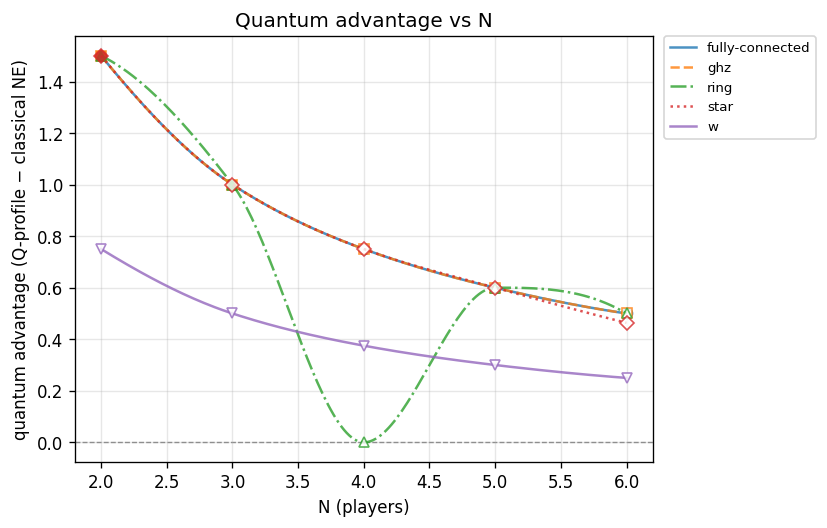
\includegraphics[width=\linewidth]{advantage_vs_N.png}
\caption{Zero-noise quantum advantage of the cooperative profile
$(Q_N,\dots,Q_N)$ over the best classical pure Nash payoff, at
$\gamma=\pi/2$ and $V{=}4, C{=}3$, versus player count $N$ for the five
entanglement topologies. The GHZ-family ideal $3/N$ (star markers) is
attained by GHZ and fully connected at every $N$; the ring dips to zero
advantage at $N=4$; the star shows a weaker $N{=}6$ deviation
($0.463$ vs.\ $0.5$); W tracks below throughout. Filled markers indicate
$(Q_N,\dots,Q_N)$ is a pure Nash equilibrium --- the fully symmetric case
holds only at $N\le3$.}
\label{fig:advmap}
% source: results/n-scaling-advantage/2026-07-19T0901Z/plots/advantage_vs_N.png
\end{figure}

\begin{figure}[t]
\centering
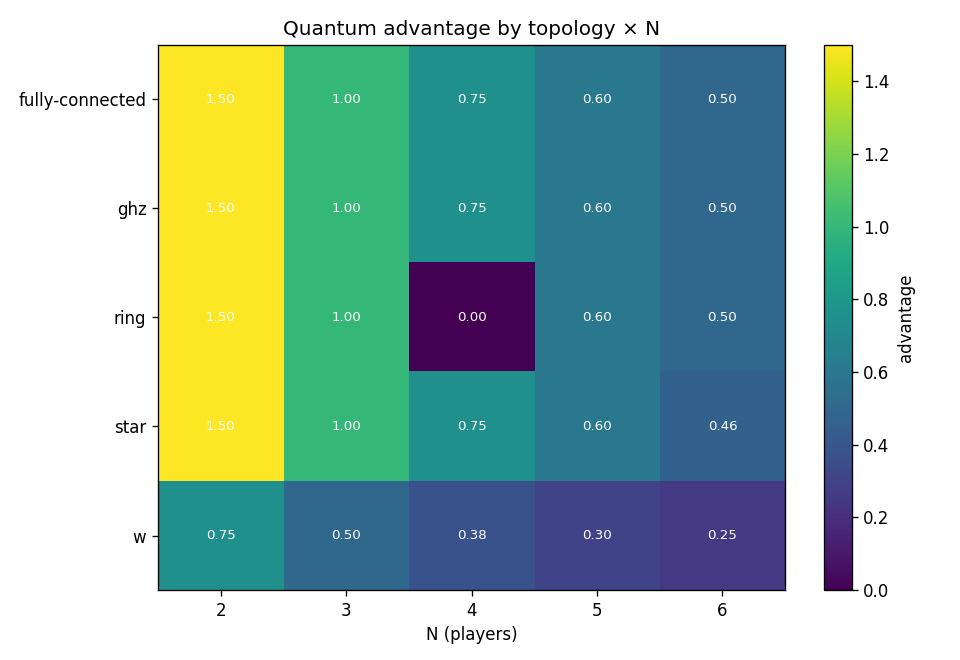
\includegraphics[width=\linewidth]{topology_heatmap.png}
\caption{Advantage heatmap across the $(N,\text{topology})$ grid at
$V{=}4, C{=}3$ (mean per-player payoff of $(Q_N,\dots,Q_N)$ minus best
classical pure Nash payoff). The GHZ/fully-connected row holds the
theoretical $3/N$ everywhere; the single dark cell is the ring at $N=4$
(advantage exactly $0$).}
\label{fig:heat}
% source: results/n-scaling-advantage/2026-07-19T0901Z/plots/topology_heatmap.png
\end{figure}

% gamma-sweep data: results/gamma-sweep/N2..N6 (V=4/C=3, fixed mode, noiseless)
Sweeping the entanglement angle $\gamma$ from $0$ to $\pi/2$ maps how much
entanglement the quantum equilibrium actually needs. At $N{=}2$ every
topology's advantage is already positive from $\gamma{=}0$ and $(Q,Q)$ becomes
a pure Nash equilibrium from $\gamma=0.3\pi$ (W excepted --- never Nash in
range). At $N{=}3$ the vertex-transitive topologies (GHZ, fully-connected,
ring) hold the full advantage $1.0$ flat across the whole sweep and become
Nash at $\gamma=0.3\pi$--$0.4\pi$; the star and W never reach a pure
equilibrium. At $N{=}4$ (Fig.~\ref{fig:gamma}) the topologies split: GHZ and
star hold the full $0.75$ at every $\gamma$, fully-connected dips to $0.40$
mid-sweep and recovers, W decays monotonically to $0.375$, and the ring
collapses to exactly zero at $\gamma=\pi/2$ --- the period-4 interference dip.
No series crosses zero advantage except that ring endpoint.

\begin{figure}[t]
\centering
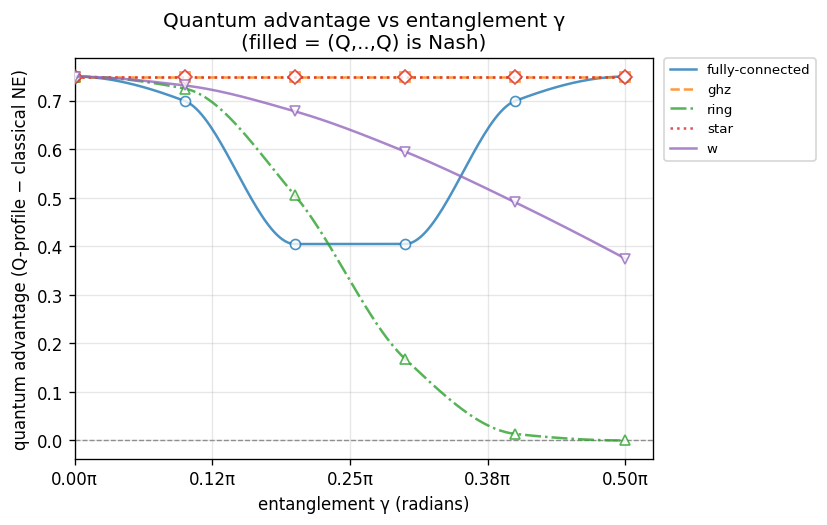
\includegraphics[width=\linewidth]{advantage_vs_gamma_N4.png}
\caption{Quantum advantage versus entanglement angle $\gamma$ at $N{=}4$
($V{=}4, C{=}3$, noiseless). GHZ and star hold the full $0.75$ flat;
fully-connected dips and recovers; W decays monotonically; the ring falls to
zero at $\gamma=\pi/2$. Data:
\texttt{results/gamma-sweep/N4}.}
\label{fig:gamma}
\end{figure}

% star per-player data: results/n-scaling-advantage/2026-07-19T0901Z/plots/per_player_advantage_star.png
The star is the only topology that breaks player symmetry at zero noise. For
$N\ge4$ the advantage is real but unevenly shared
(Fig.~\ref{fig:star}): at $N{=}4$ the three leaves gain $1.0$ each while the
hub gains nothing ($0.0$); by $N{=}6$ the hub gains $0.952$ against the
leaves' $0.366$. The mean stays close to the theoretical $3/N$ until $N{=}6$,
where the hub--leaf split pulls it to $0.463$.

\begin{figure}[t]
\centering
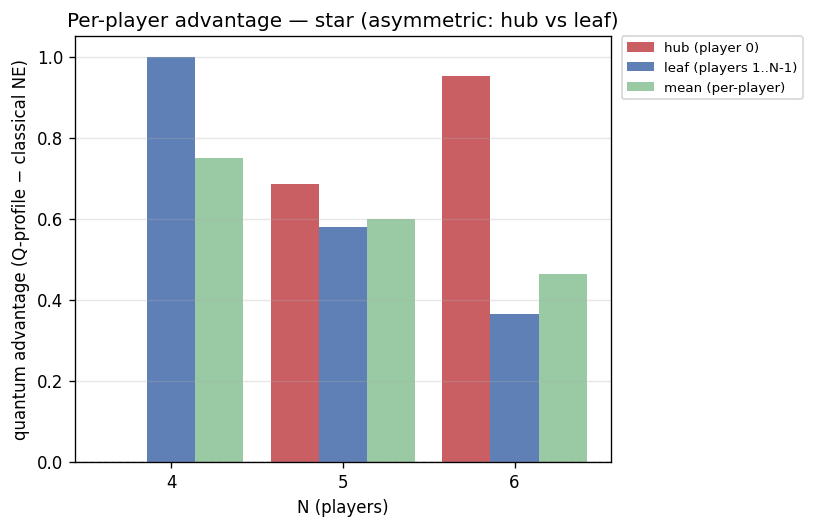
\includegraphics[width=\linewidth]{per_player_advantage_star.png}
\caption{Star-topology per-player advantage (hub player 0 vs.\ each leaf) at
$\gamma=\pi/2$, $V{=}4, C{=}3$, noiseless, for $N=2\ldots6$. The leaves
capture the advantage at small $N$; the hub captures it at large $N$; the
mean (dashed) tracks $3/N$ until $N{=}6$. Data:
\texttt{results/n-scaling-advantage/2026-07-19T0901Z}.}
\label{fig:star}
\end{figure}

\subsection{Noise robustness: two criteria disagree}\label{sec:noise}
% ported from README §9 (Month-4, corrected 2026-07-17); data results/noise-robustness/2026-07-03T0213Z
Sweeping the depolarizing strength $p$ from $0$ to $0.05$ on the gate-level
noisy path, two natural ``robustness'' criteria give different orderings, so
we state which we mean. Under the \emph{Nash-equilibrium} criterion, the GHZ
cooperative profile is fragile: $(Q,\dots,Q)$ is a pure equilibrium at $p=0$
only for GHZ $N{=}2,3$, and at $N{=}3$ it loses equilibrium status between
$p=0.04$ and $0.045$. For $N{=}4,5$ the GHZ thresholds $p^*\approx0.0197$
and $0.0098$ are \emph{advantage-zero crossings}, not equilibrium losses ---
$(Q,\dots,Q)$ is not a pure equilibrium there even at $p=0$. For W and ring
the fixed GHZ-derived $Q$ is never a strict pure equilibrium even at $p=0$,
so the equilibrium criterion does not apply.

Under the \emph{advantage-magnitude} criterion the picture flips: at $N{=}3$
GHZ retains the most mean advantage at $p=0.05$ ($0.333$, $33\%$ of its
noiseless value) versus ring $0.200$ and W $0.047$. So ``GHZ degrades
fastest'' holds for the equilibrium, not for advantage magnitude at small
$N$. This ordering is a property of the production circuits at their gate
budgets: gate-count-matched controls show per-$cx$ advantage decay rates are
indistinguishable across GHZ/ring/star/fully-connected ($\lambda/cx\approx
2.1$--$2.7$), while W is the genuine structural outlier at $\approx2.5\times$
more robust \emph{per gate} ($\lambda/cx\approx0.8$--$1.0$). W keeps a
positive-but-small mean advantage across the whole grid, but the mean hides
per-player losses: at $N{=}5$ two of the five players have negative
advantage from $p=0.01$ (worst $-0.077$ at $p=0.015$). All entanglers here
are exact gate-level circuits; W uses the T8 construction (44 and 68 $cx$
per $J$ at $N{=}4,5$, versus $100$/$444$ for the retired transpiled-unitary
fallback).

\subsection{Position-locked unfairness and the adaptation pilot}
% wiring-permutation: README §9 Month-4 findings; T9 pilot: docs/findings/2026-07-05-t9-adaptation-fairness.md
The noise-induced per-player asymmetry is not a property of the player labels
or the ideal state. A wiring-permutation test on the ring at $N{=}5$
(\texttt{scripts/asymmetry\_diagnostics.py}) cyclically shifts the
qubit-to-player wiring and the whole per-player payoff vector permutes
rigidly with it (deviation $\sim10^{-16}$); and applying the same depolarizing
weight to the \emph{ideal final state} instead of per-gate collapses the
per-player spread to $\sim0$. The disadvantage therefore follows the
entangler's \emph{circuit position} (gate ordering), not the ideal state or
the player identity.

An exploratory W-state pilot ($N{=}4$) then asks whether letting each player
independently best-respond under the same noisy circuit repairs the
unfairness. It does not beneficially do so at any noise level tested: at
$p{=}0$ adaptation equalizes only by collapsing collective welfare (mean
$1.00\rightarrow0.51$); at $p{=}0.02$ the best-response dynamics fail to
converge, settling on a payoff limit cycle whose time-averaged state is both
less fair (spread $0.014\rightarrow0.036$) and lower-welfare (mean
$0.98\rightarrow0.88$) than the fixed cooperative baseline; at $p{=}0.05$ it
converges but changes almost nothing. The adaptation rule (independent
round-robin best response) is provisional pending game-theory sign-off, so
this is a directional finding, not a locked result --- but it is consistent
with the position-locked mechanism: the fairness loss is structural to the
circuit, not a coordination failure that self-interested play adapts away.

% =============================================================================
\section{Hardware Validation on IBM Heron r2}\label{sec:hardware}

\subsection{Pipeline and safeguards}
Every submission passes three gates: (i) an $\mathrm{Operator.equiv}$
circuit-identity assertion against the dense
$J^\dagger (U^{\otimes N}) J$ reference, (ii) a noiseless simulator dry-run
that must reproduce the exact analytic advantage, and (iii) a full dress
rehearsal of the batch --- including mitigation analysis --- on the device
noise model reduced to the executed qubits. Job identifiers are persisted
before result polling, making runs crash-safe and recoverable.
% experiments/hardware_scaling.py; spec docs/superpowers/specs/2026-07-16-*.md

\subsection{Single-point validation at $N=3$}
% results/hardware-n3/2026-07-16T013912Z/ (job d9br6l66hjac73fg3g7g)
The validated $Q_3$ circuit (entangler decomposed to 6 native cz gates) run
with 4096 shots on ibm\_fez measured advantage $0.9978$ against the ideal
$1.0$, with $3911/4096$ shots in $\ket{000}$
(Fig.~\ref{fig:n3}).

The error budget is consistent with an independent-error picture once the
observable's structure is taken into account. Multiplying the three
calibrated single-shot readout fidelities ($0.9960$, $0.9961$, $0.9962$) by
the six two-qubit-gate fidelities (edge errors $0.17\%$ and $0.23\%$ over
the entangler's two edges) predicts a ground-state probability of
$\approx 0.977$, modestly above the measured $0.955$; the per-edge split of
the six \textsc{cz} gates moves this by less than $0.002$.
% run: results/hardware-n3/2026-07-16T013912Z job d9br6l66hjac73fg3g7g;
% readout_error 136/143/142, twoq_gate_error 136_143 / 143_142;
% p_naive = prod(1-r_i) * (1-g_a)^4 (1-g_b)^2 = 0.9771 (4+2), 0.9765 (3+3)
What the naive budget does not predict is the payoff: the same run's mean
payoff is $0.9978$ of ideal, not $95\%$ of it. The measured counts show why.
Of the $185$ shots outside $\ket{000}$, $176$ ($95\%$ of the error weight)
land on one- and two-Hawk outcomes, whose per-player payoffs still average
$V/N$ --- the Hawk captures $V$ in full, so the mean is unchanged --- and
only the $9$ all-Hawk shots ($0.22\%$) reduce the mean, to $(V-C)/N$.
% counts: k=0:3911, k=1:53, k=2:123, k=3:9 (result.json counts block);
% k<3 mean V/N, k=3 mean (V-C)/N -> reconstructed mean 1.331136 = measured
The mean-payoff observable is therefore first-order insensitive to single
bit-flips from the ideal outcome: errors that flip one qubit redistribute
payoff between players without lowering its mean. This is the structural
mechanism behind the scaling section's central observation --- the advantage
decays several times slower than the state fidelity --- and it is why the
$N{=}3$ advantage survives at $0.998$ while $P(\ket{000})$ has already lost
$4.5\%$.

\begin{figure}[t]
  \centering
  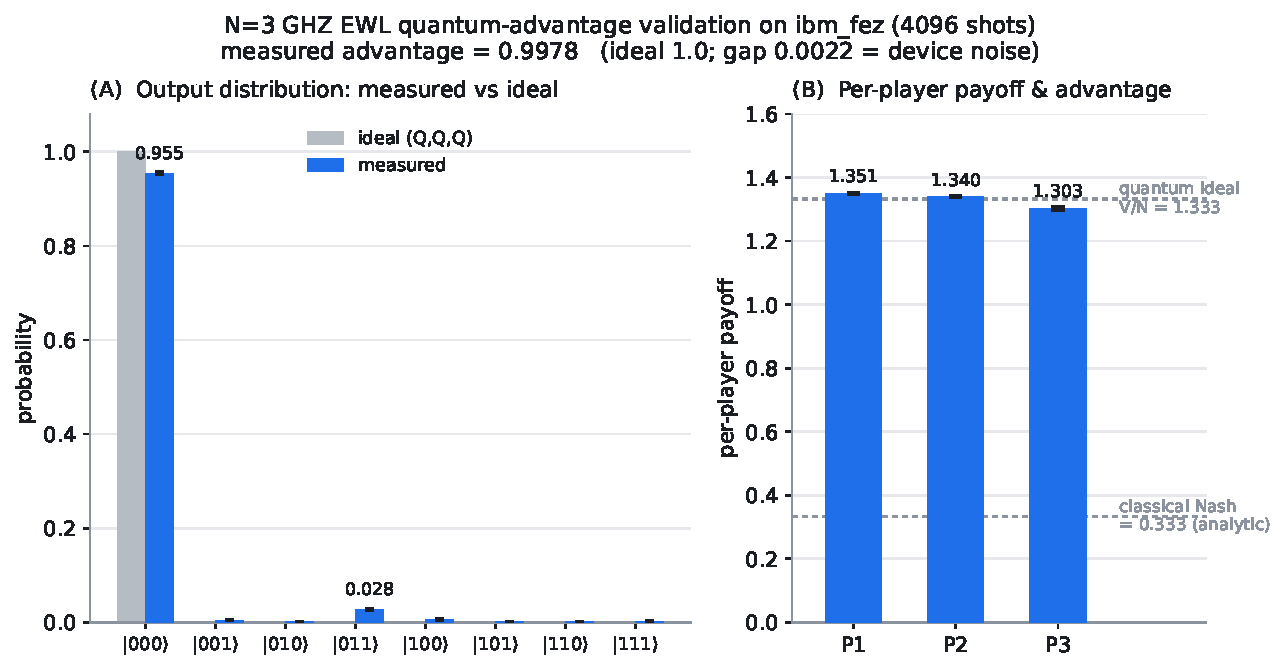
\includegraphics[width=\linewidth]{hardware_n3_validation.pdf}
  \caption{Hardware validation of the $N{=}3$ GHZ EWL quantum advantage on
  ibm\_fez (IBM Heron r2). The validated $(Q,Q,Q)$ circuit --- entangler $J$
  decomposed to 6 native cz gates --- was executed with 4096 shots.
  \textbf{(A)} Measured output distribution over the eight
  computational-basis states (blue) versus the noiseless ideal (grey); error
  bars are binomial shot noise. $3911/4096$ shots (95.5\%) fall in
  $|0\ldots0\rangle$, the ideal $(Q,Q,Q)$ output. \textbf{(B)} Measured
  per-player payoff (blue) against the analytic classical-Nash baseline
  ($0.333$, noiseless) and the quantum ideal $V/N=1.333$; error bars
  propagate shot noise. The measured mean payoff $1.331$ gives advantage
  $0.9978$ vs the ideal $1.0$. Physical qubits $\{136,143,142\}$ (calibration
  2026-07-15): readout error 0.38--0.40\%, cz error 136--143: 0.17\%,
  143--142: 0.23\%.}
  \label{fig:n3}
\end{figure}

\subsection{Scaling at $N=3,4,5$ with error mitigation}
% results/hardware-scaling/2026-07-16T074134Z/ (job d9c8fpn550hc73dl1tcg)
All three $N$ ran on prefixes of one pinned 5-qubit chain
$[59,75,74,73,79]$ (chosen by calibration error) in a single 11-pub batch:
two readout-calibration circuits plus $N\in\{3,4,5\}\times$ cz-fold
$\lambda\in\{1,3,5\}$. Readout errors are corrected by tensored confusion-matrix
inversion (constrained least squares)~\cite{nation2021}; zero-noise
extrapolation folds each cz locally ($\mathrm{cz}\to\mathrm{cz}^\lambda$,
unitary-preserving since cz is self-inverse) and extrapolates the
readout-mitigated payoff linearly to $\lambda=0$~\cite{temme2017,kandala2019}.

\begin{table}[t]
\centering
\caption{Measured advantage on ibm\_fez (4096 shots; single run --- repeats in
progress). Ideal advantage is $3/N$; retention is ZNE/ideal.}
\label{tab:scaling}
\begin{tabular}{@{}ccccc c@{}}
\toprule
$N$ & ideal & raw & mitig.+ZNE & retention & $P(\ket{0\ldots0})$\\
\midrule
3 & 1.00 & 0.9919 & 0.9938 & 99.4\% & 0.938\\
4 & 0.75 & 0.7386 & 0.7403 & 98.7\% & 0.922\\
5 & 0.60 & 0.5837 & 0.5887 & 98.1\% & 0.868\\
\bottomrule
\end{tabular}
\end{table}

\begin{figure*}[t]
  \centering
  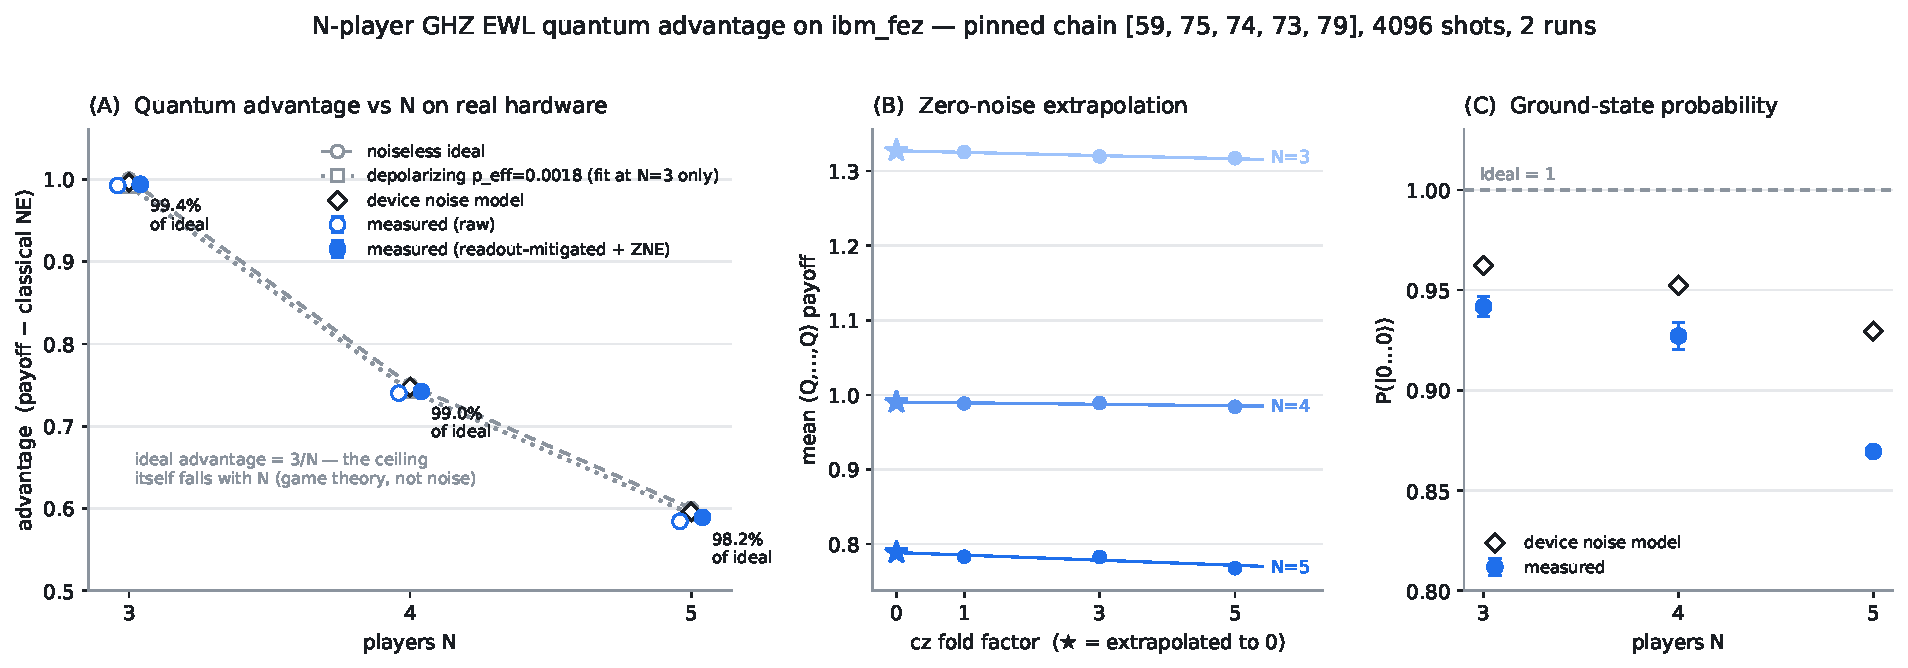
\includegraphics[width=\textwidth]{hardware_scaling.pdf}
  \caption{Scaling of the $N$-player GHZ EWL quantum advantage on ibm\_fez
  (IBM Heron r2), physical chain $[59,75,74,73,79]$, 4096 shots.
  \textbf{(A)} Measured cooperative-profile advantage (mean $(Q,\ldots,Q)$
  payoff minus the analytic noiseless classical-Nash payoff) at $N=3,4,5$:
  raw (open) and readout-mitigated $+$ ZNE (filled), against the noiseless
  ideal ($1.0, 0.75, 0.6$), the device noise-model prediction (diamonds), and
  a single-parameter depolarizing model with $p_{\mathrm{eff}}=0.0018$ fitted
  to the $N{=}3$ point alone --- its $N{=}4,5$ values are predictions, not
  fits. Error bars: multinomial shot noise (raw) and weighted-fit standard
  error (ZNE). \textbf{(B)} ZNE mechanics: readout-mitigated payoff vs cz
  fold factor ($\lambda=1,3,5$) with the weighted linear fit extrapolated to
  $\lambda=0$ (stars). \textbf{(C)} Ground-state probability
  $P(|0\ldots0\rangle)$: the state fidelity decays several times faster than
  the advantage because the mean-payoff observable is first-order insensitive
  to single bit-flips from $|0\ldots0\rangle$. $(Q,\ldots,Q)$ is a pure Nash
  equilibrium only at $N{=}3$; at $N{=}4,5$ the profile is the cooperative
  quantum profile, not an equilibrium. Calibration 2026-07-16; job
  d9c8fpn550hc73dl1tcg.}
  \label{fig:scaling}
\end{figure*}

Two model predictions frame
Table~\ref{tab:scaling}: the reduced device noise model
(\texttt{NoiseModel.from\_backend}) and a \emph{fit-one-predict-two} test in
the paper's own depolarizing model --- a single $p_{\text{eff}}=0.0018$
fitted to the $N{=}3$ mitigated point, committed as the registered primary
prediction before any repeat run. It predicts $N{=}4$ to $0.004$; at $N{=}5$
it over-predicts by $0.010$ ($\approx$5$\sigma$ of the registered predictive
interval), a deficit that reproduces on a second run. In the registered
five-model comparison, an exponential-retention baseline in the transpiled
two-qubit-gate count leads both runs, so we treat per-gate decay as the
operative scaling law and $p_{\text{eff}}$ as its physical interpretation.
% registered: results/hardware-scaling/preregistration.json and
% preregistration-baselines.json; outcomes:
% results/hardware-scaling/repeat-judgments.json
% (run 1: cz 10.0 vs p_eff 31.3; run 2: cz 7.4 vs p_eff 23.4)

\subsection{Why the advantage outlives the state}
Ground-state probability decays $\sim$3$\times$ faster than the advantage
(Table~\ref{tab:scaling}): a single bit-flip from $\ket{0\ldots0}$ yields a
one-Hawk outcome whose \emph{mean} payoff is still exactly $V/N$, so the
mean-payoff observable is first-order insensitive to uncorrelated single
flips. Readout mitigation consequently moves the mean very little (it mainly
repairs \emph{per-player} fairness), while ZNE --- targeting the correlated cz
errors that create $\ge$2-Hawk outcomes --- improves every series. This
structural robustness is a property of the game's payoff geometry, not of the
device.

The same single-flip terms that leave the mean invariant are what create
winners and losers. Under the all-Dove branch each one-Hawk outcome transfers
$V$ to a single player and zero to the rest: the mean is protected, the
individual player is not, and under gate-level noise the disadvantaged
position is locked to the entangler's circuit layout rather than to any
coordination failure (Sec.~\ref{sec:noise}).
% docs/findings/2026-07-05-t9-adaptation-fairness.md; ring N=5 permutation
% test scripts/asymmetry_diagnostics.py (README \S9 Month-4 findings)
An exploratory W-state pilot finds the asymmetry is not repaired by
self-interested play: letting each player independently best-respond either
equalizes only by collapsing the group mean ($1.00 \rightarrow 0.51$ at
$p{=}0$) or fails to converge at all (a payoff limit cycle at $p{=}0.02$).
The adaptation rule is provisional and this is not a locked finding, but the
direction is consistent --- the fairness loss is structural to the circuit,
not an artifact players adapt away. The advantage we report is therefore a
mean over players who do not share it equally; the per-player floor, not the
mean, is the quantity a mechanism designer should optimize.

% =============================================================================
\section{Discussion}\label{sec:discussion}

% market interpretation: README §10
The topology sweep is a market-design map: each entanglement pattern
corresponds to a connectivity architecture, and the results say which
architecture sustains cooperation. A centralised order book is a star; OTC
derivatives and interdealer networks are ring or partially-connected; a dense
interbank market is fully-connected. The two-criteria dichotomy of
Sec.~\ref{sec:noise} yields a concrete design rule: choose the topology by
whether the mechanism needs the \emph{equilibrium} or the \emph{payoff}. If
the goal is a self-enforcing cooperative equilibrium that survives noise, GHZ
at small $N$ is the only topology that delivers one --- but it is fragile,
losing equilibrium status at finite $p$. If the goal is a large, durable
cooperative payoff (accepting a fixed protocol rather than an equilibrium),
GHZ again leads at small $N$ on advantage magnitude, while W's superior
per-gate robustness makes it the choice when two-qubit gates --- not
entanglement structure --- are the binding constraint. Two applications make
the mapping concrete. In carbon markets (an $N$-player Hawk--Dove between
emission reduction and allowance purchase), the topology that maximises
cooperative payoff at a given noise budget is the optimal architecture for a
quantum-enhanced trading mechanism. In DeFi, where front-running (MEV) is an
$N$-player Hawk--Dove that destroys value, entangling wallet interactions via
a smart-contract-controlled quantum channel could enforce cooperative
outcomes without a trusted intermediary --- the entanglement graph maps
directly onto the contract-interaction graph.

\textbf{Limitations.} Discrete strategy set $\{D,H,Q_N\}$ (mixed/continuous
deviations are future work); the fixed GHZ-derived $Q_N$ is not
topology-optimized under noise; hardware results are from one device, one
chain, and (currently) one calibration day --- the repeat protocol is running
and Table~\ref{tab:scaling} gains cross-day error bars as runs accumulate;
the T9 adaptation rule is provisional.

% =============================================================================
\section{Conclusion}\label{sec:conclusion}
We asked whether the two-player quantum Hawk--Dove advantage survives the
transition to real $N$-player networks --- topologies, noise, and hardware.
The landscape is now charted, and the answer is yes, with sharper edges than
the two-player picture suggests. At $N{=}3$ the GHZ cooperative profile is a
genuine symmetric pure Nash equilibrium, and it reproduces on superconducting
hardware within $0.2\%$ of the noiseless ideal ($0.9978$ of ideal, job
\texttt{d9br6l66hjac73fg3g7g}).
% results/hardware-n3/2026-07-16T013912Z/result.json (measured_advantage 0.9978)
At $N{=}4,5$ the same profile ceases to be an equilibrium --- a unilateral
Hawk deviation profits --- yet its cooperative payoff retains a large,
measurable advantage over the analytic classical baseline on the same device
($0.739 / 0.584$ of the ideal $0.75 / 0.60$).
% results/hardware-scaling/2026-07-16T074134Z and 2026-07-17T014458Z
The dichotomy --- equilibrium at $N{=}3$, cooperative profile beyond --- is
real, and it is a feature of the game, not a defect of the experiment.

Three structural findings carry the design weight. First, the mean-payoff
observable is first-order insensitive to single bit-flips, so the advantage
decays several times slower than the state fidelity: quantum market
mechanisms degrade gracefully on NISQ devices. Second, the same flip terms
that spare the mean concentrate loss on individual players --- a fairness
cost that self-interested adaptation does not repair --- so the quantity a
mechanism should optimize is the per-player floor, not the mean. Third, the
scaling of the advantage with $N$ is set not by a fitted depolarizing
strength but by per-two-qubit-gate decay: in the registered five-model
comparison an exponential-retention law in the transpiled \textsc{cz} count
leads both hardware runs, with the depolarizing fit surviving as its physical
interpretation.
% results/hardware-scaling/repeat-judgments.json

The limitations are the same honesty notes threaded through the text: the
$N{=}4,5$ curve measures a fixed cooperative protocol, not an equilibrium;
the hardware numbers are single-calibration-day results with cross-day
repeats in progress; and the fairness link rests on an exploratory adaptation
rule. Within those bounds the design implication is concrete --- entanglement
topology is a market-design variable whose noise cost is budgeted per
two-qubit gate, and its benefit should be read at the per-player floor.

\section*{Reproducibility}
All circuits, harnesses, per-run calibration snapshots, and analysis code are
open source at \url{https://github.com/Prithvi8706/Multiplayer-QHD-Game}
(pinned qiskit 1.3.2 / qiskit-aer 0.14.2 / qiskit-ibm-runtime 0.36.1); every
hardware artifact records its job id, chain, and calibration.

\bibliographystyle{IEEEtran}
\bibliography{references}

\end{document}
